
\section{The facts of (numerical) life}

Our goal is to compute more interesting quantities than Euler's constant $e$.  At the core of most \PETSc computations, and many numerical PDE solutions, is a finite-dimensional linear system.  In this section we both recall basic ideas of numerical linear algebra and apply \PETSc to solve simple linear systems.

Suppose $\bb\in \RR^{N}$ is a column vector and $A\in\RR^{N\times N}$ is a square matrix.\sidenote{\PETSc can handle complex matrices, but all matrices are real in this book.}  The linear system
\begin{equation}
A \bu = \bb \label{introsystem}
\end{equation}
has a unique solution $\bu\in \RR^{N}$ if $A$ is invertible, namely
\begin{equation}
\bu = A^{-1} \bb. \label{introsolution}
\end{equation}
This is simple in theory.

It is not so simple in practice, however, to solve linear systems on a computer.  Here are two facts to keep in mind while working numerically with linear systems \citep{TrefethenBau}:
\renewcommand{\labelenumi}{\roman{enumi})}
\begin{enumerate}
\item \label{limittoaccuracy} \emph{limit to accuracy}:  If real numbers are represented with machine precision $\eps$ then the solution of \eqref{introsystem} can only be computed within an error $\kappa(A) \eps$ where $\kappa(A) = \|A\| \|A^{-1}\|$ is the \emph{condition number} of $A$ (for the induced matrix norm $\|\cdot\|$).
\item \emph{cost of direct solutions}:  If $A$ is a generic $N\times N$ matrix then computation of solution \eqref{introsolution} by a direct method, like Gauss elimination, whether actually forming $A^{-1}$ or not, is an $O(N^3)$ operation.
\end{enumerate}

Fact i) is about conditioning not methods.  Informally speaking, there are matrices $A$ and $\tilde A$ that are the same to within $\eps$ but for which the infinite-precision solutions to \eqref{introsolution} differ by an amount $\kappa(A) \eps$.  Rounding errors, which is like random noise added to every arithmetic operation on the computer, act to perturb $A$ by $\eps$ during any computation, and thus at least $\kappa(A) \eps$ size errors appear in the solution of the linear system.  However, \emph{backward stable} direct methods, specifically the QR method, can be shown to actually achieve this level of accuracy on all matrices.

The precision for the C \texttt{double} type, the default 64-bit representation of real numbers, a type aliased to \texttt{PetscReal} in our \PETSc programs, is $\eps = 2.2 \times 10^{-16}$.  Thus by i), a linear system having $\kappa(A) \approx 10^{10}$, for example, can only be solved to five or six decimal digits of precision.  While a matrix with such a large condition number is ``poorly-conditioned,'' it is possible to reach that level for $\kappa(A)$ when discretizing PDEs.  We have to be aware of conditioning when forming expectations about solution accuracy.

By ii) a generic linear system with $N=10^6$ equations requires $10^{18}$ or so operations to solve by Gauss elimination.  Even modern supercomputers take a while to do a quintillion operations.  However, though general-purpose direct methods are impractical for $N=10^6$ systems, we will successfully solve PDE-generated linear systems of this size on a single processor in a few seconds, and in $O(N)$ operations, in Chapter \ref{chap:multigrid}.  The key fact is that discretized PDEs generate linear systems with exploitable structure, especially \emph{sparsity}, namely only a few nonzero entries per matrix row.  For the methods to converge there needs to be other structure, such as regularity of the matrix entries arising from the smoothness of the coefficients in the PDE.  In any case, this structure will must be exploited, and exposed to one degree or another, in serious numerical PDE solutions.  Naive application of direct methods---treating solvers for \eqref{introsystem} as unadjusted black boxes---is too slow.
%ch5/:  timer ./fish2 -da_refine 7 -ksp_type cg -pc_type mg
%on 1153 x 1153 grid:  iterations 2, residual norm = 1.88082e-05
%real 11.18

It is reasonable to add one more point about computer memory, not operation count, to our above list of facts-of-life:
\begin{enumerate}
\item[iii)] \emph{do not form the inverse}:  The matrices $A$ arising from discretized PDEs are usually sparse, but their inverses $A^{-1}$ are usually dense and may not even fit in computer memory.
\end{enumerate}

The difference in memory cost can be dramatic.  For example, the $N$-dimensional tridiagonal matrix $A$ assembled later in this section occupies $24 N$ bytes, because each allocated real entry occupies 8 bytes using \texttt{double} precision.  The inverse $A^{-1}$, however, is dense and uses $8 N^2$ bytes.  Though we can easily solve $A\bu=\bb$ for this matrix in dimension $N=10^7$, in a few seconds on a single processor using less than a gigabyte of memory in the solution process,\sidenote{See \texttt{tri.c}.  Do ``\texttt{tri -tri\_m 10000000 -ksp\_type cg -pc\_type none}.''} simply storing $A^{-1}$ would occupy $800$ terabytes of memory or disk.
\vfill


\section{\PETSc \pVec and \pMat objects}

To build our first \PETSc code to solve a linear system, we need the \emph{objects} which hold vectors and matrices.  Note that, although \PETSc is written in C and not C++, for example, it is a relentlessly object-oriented software library.  Consider the operations which create and configure a matrix object \texttt{A} for linear system \eqref{introsystem}:
\begin{code}
Mat A;
MatCreate(COMM,&A);
MatSetSizes(A,PETSC_DECIDE,PETSC_DECIDE,N,N);
MatSetOptionsPrefix(A,"a_");
MatSetFromOptions(A);
... fill entries of (i.e. assemble) A ...
... solve system with A ...
MatDestroy(&A);
\end{code}
We can think of these calls as methods ``owned'' by the \pMat type, in the sense that they manipulate the internal representation of a \pMat, which is hidden.  If not true ``objects'', major \PETSc types are at least abstract data types with a hidden implementation.

Methods for filling entries of \pMat objects will treat them abstractly too.  In fact, a \pMat need not even have entries.  It might, instead, contain code that applies a linear operator to vectors.  Furthermore the data structure inside a \pMat depends on runtime choices, the most basic being that the number of bytes used to store matrix entries on a given MPI process will depend on the number of processes.

In the code above, note the call to \texttt{MatSetOptionsPrefix()}.  Through the prefix, run-time options can address the particular \pMat object.  For example, the run-time option \texttt{-a\_mat\_view} will print out the entries of \texttt{A}.  We can distinguish multiple \pMat objects at the command line by their prefixes.

Once \pMat \texttt{A} is created and set up by the first several commands \texttt{MatCreate()}--\texttt{MatSetFromOptions()}, then various methods become valid for \texttt{A}, for example including the \texttt{MatSetValues()} method to set entries in \texttt{A}.
 
This sequence of operations applies to all \PETSc object types:
\begin{code}
Object X;
ObjectCreate(COMM,&X);
... code sets properties of X ...
ObjectSetFromOptions(X);  // allows run-time setting
                          // or overriding of properties
... code uses X ...
ObjectDestroy(&X);
\end{code}
Because \PETSc objects are generally distributed across, and accessible from, multiple MPI processes, the first argument of an \texttt{ObjectCreate()} method is an MPI communicator (``\texttt{COMM}'').  We will usually use \texttt{PETSC\_COMM\_WORLD}; it is the default communicator formed from all \texttt{N} processes when we start a run with ``\texttt{mpiexec -n N}.''  Because they are ``collective'' operations, all processes in \texttt{COMM} must call the \texttt{ObjectCreate()} and  \texttt{ObjectDestroy()} methods.


\section{Assembly and parallel layout of \pVecs and \pMats}

A \pVec or \pMat stores its entries in parallel across all the processes in the MPI communicator used when creating it.  For example, the create-assemble sequence of a \pVec with four entries might look like this:
\begin{code}
Vec x;
PetscInt   i[4] = {0, 1, 2, 3};
PetscReal  v[4] = {11.0, 7.0, 5.0, 3.0};

VecCreate(COMM,&x);
VecSetSizes(x,PETSC_DECIDE,4);
VecSetFromOptions(x);
VecSetValues(x,4,i,v,INSERT_VALUES);
VecAssemblyBegin(x);
VecAssemblyEnd(x);
\end{code}
The four entries of \texttt{Vec x} are set by \texttt{VecSetValues()}, putting values from array \texttt{v} at the indices given by \texttt{i}.  The operation of setting values in \texttt{x} may require communication between processes, however, because entries which are to be stored on one process could be set by another process.  Such communication occurs between the \texttt{VecAssemblyBegin()} and \texttt{VecAssemblyEnd()} commands.

\begin{marginfigure}
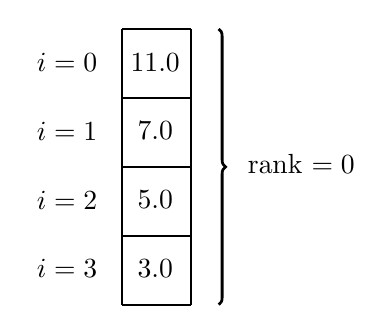
\begin{tikzpicture}[scale=3.5]
  \pgfmathsetmacro\fourth{1.0/4.0}
  \pgfmathsetmacro\xoff{0.12}
  \pgfmathsetmacro\yoff{0.12}
  \draw[xstep=\fourth,ystep=\fourth,black,thick] (0.0,0.0) grid (\fourth,1.0);
  \node at (-0.2,1.0-\yoff) {$i=0$};
  \node at (\xoff,1.0-\yoff) {$11.0$};
  \node at (-0.2,0.75-\yoff) {$i=1$};
  \node at (\xoff,0.75-\yoff) {$7.0$};
  \node at (-0.2,0.5-\yoff) {$i=2$};
  \node at (\xoff,0.5-\yoff) {$5.0$};
  \node at (-0.2,0.25-\yoff) {$i=3$};
  \node at (\xoff,0.25-\yoff) {$3.0$};
  \draw[decoration={brace,mirror,raise=5pt},decorate,line width=1pt] (0.3,0.0) -- (0.3,1.0);
  \node at (0.65,0.51) {rank $=0$};
\end{tikzpicture}
\bigskip
\caption{A sequential \pVec layout, all on rank $=0$ process.}
\label{fig:seqveclayout}
\end{marginfigure}

The reader is allowed to think of a \PETSc \pVec as a one-dimensional C array with its contents split across the processes in the MPI communicator used in the \texttt{VecCreate()} command.  For example, if the above code appears in \texttt{mycode.c}, and if it is run sequentially on one process, i.e.~as
\begin{cline}
$ ./mycode.c
\end{cline}
%$
then, at the end of the above create-set-assemble sequence, the storage of \texttt{x} looks like Figure \ref{fig:seqveclayout}.  However, if run as
\begin{cline}
$ mpiexec -n 2 ./mycode.c
\end{cline}
%$
then the layout looks like Figure \ref{fig:mpitwoveclayout}.  In this case the argument \texttt{PETSC\_DECIDE} in \texttt{VecSetSizes()} is active, and the decision is to put the first two entries of \texttt{x} on the rank $0$ process and the other two on the rank $1$ process. 

\begin{marginfigure}
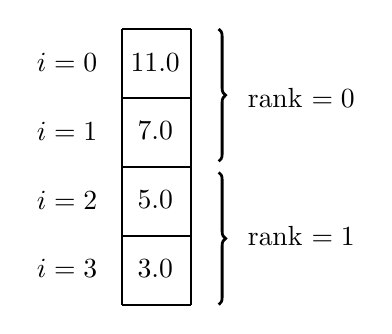
\begin{tikzpicture}[scale=3.5]
  \pgfmathsetmacro\fourth{1.0/4.0}
  \pgfmathsetmacro\xoff{0.12}
  \pgfmathsetmacro\yoff{0.12}
  \draw[xstep=\fourth,ystep=\fourth,black,thick] (0.0,0.0) grid (\fourth,1.0);
  \node at (-0.2,1.0-\yoff) {$i=0$};
  \node at (\xoff,1.0-\yoff) {$11.0$};
  \node at (-0.2,0.75-\yoff) {$i=1$};
  \node at (\xoff,0.75-\yoff) {$7.0$};
  \node at (-0.2,0.5-\yoff) {$i=2$};
  \node at (\xoff,0.5-\yoff) {$5.0$};
  \node at (-0.2,0.25-\yoff) {$i=3$};
  \node at (\xoff,0.25-\yoff) {$3.0$};
  \draw[decoration={brace,mirror,raise=5pt},decorate,line width=1pt] (0.3,0.52) -- (0.3,1.0);
  \node at (0.65,0.752) {rank $=0$};
  \draw[decoration={brace,mirror,raise=5pt},decorate,line width=1pt] (0.3,0.0) -- (0.3,0.48);
  \node at (0.65,0.251) {rank $=1$};
\end{tikzpicture}
\bigskip
\caption{A parallel \pVec layout on two processes.  Because we call ``\texttt{VecSetSizes(x,PETSC\_DECIDE,4)}'', \PETSc decides to split the storage in the middle.}
\label{fig:mpitwoveclayout}
\end{marginfigure}

However, \pMat objects are not merely 2D C arrays even in serial (i.e.~in one-process runs).  Compared to \pVecs they require additional choices regarding parallel distribution.  Though this is hidden inside the implementation of \pMat, the most common storage format is \emph{parallel compressed sparse row storage}, what \PETSc calls the \texttt{MATMPIAIJ} type.  In this type a range of rows is owned by each process (parallel row storage), and within each owned range of rows only the specifically-allocated\sidenote{These are generally the nonzero entries, and usually referred-to as such.} entries are stored (sparse), and furthermore nonzero entries are stored contiguously in memory using an additional index array (compressed).

\pMat objects are linear operators and their major ``purpose'' is to multiply \pVecs.  The result vector of a \pMat-\pVec product is a linear combination of the columns of the \pMat.  Thus, in practice, parallel row storage of the \pMat means these things:
\begin{itemize}
\item \PETSc internally distributes the rows of the \pMat $A$ the same way as the entries of the intended \emph{output} (i.e.~column) \pVec.  Thus if $Ax=b$ for some $x$ then row $i$ of $A$ is on the rank $m$ processor if and if entry $i$ of $b$ is on the rank $m$ processor.\sidenote{This is the outcome when \texttt{PETSC\_DECIDE} is used in setting both the \pVec and \pMat sizes and they are of the same dimension.}
\item Before \PETSc computes a \pMat-\pVec product, \PETSc communicates (``scatters'') the whole \pVec to each process.
\item After the scatter the \pMat-\pVec product is a local operation, requiring no further communication.
\end{itemize}

But one doesn't really need to know all this to assemble a matrix.  For example, here is one way to create and assemble a $4\times 4$ \pMat object one row at a time:
\begin{code}
Mat A;
PetscInt  i, j[4] = {0, 1, 2, 3};
PetscReal v[4];

MatCreate(PETSC_COMM_WORLD,&A);
MatSetSizes(A,PETSC_DECIDE,PETSC_DECIDE,4,4);
MatSetFromOptions(A);
MatSetUp(A);

i = 0;  v[0] = 1.0;  v[1] = 2.0;  v[2] = 3.0;
MatSetValues(A,1,&i,3,j,v,INSERT_VALUES);
i = 1;  v[0] = 2.0;  v[1] = 1.0;  v[2] = -2.0;  v[3] = -3.0;
MatSetValues(A,1,&i,4,j,v,INSERT_VALUES);
i = 2;  v[0] = -1.0;  v[1] = 1.0;  v[2] = 1.0;  v[3] = 0.0;
MatSetValues(A,1,&i,4,j,v,INSERT_VALUES);
j[0] = 1;  j[1] = 2;  j[2] = 3;
i = 3;  v[0] = 1.0;  v[1] = 1.0;  v[2] = -1.0;
MatSetValues(A,1,&i,3,j,v,INSERT_VALUES);

MatAssemblyBegin(A,MAT_FINAL_ASSEMBLY);
MatAssemblyEnd(A,MAT_FINAL_ASSEMBLY);
\end{code}
The method \texttt{MatSetValues()} sets multiple values, in this case a row.  The ``\texttt{1,\&i}'' arguments to \texttt{MatSetValues()} say that we are setting one row with global index \texttt{i}.  The ``\texttt{3,j}'' or ``\texttt{4,j}'' arguments say that integer array \texttt{j} has the 3 or 4 global column indices.

\begin{marginfigure}
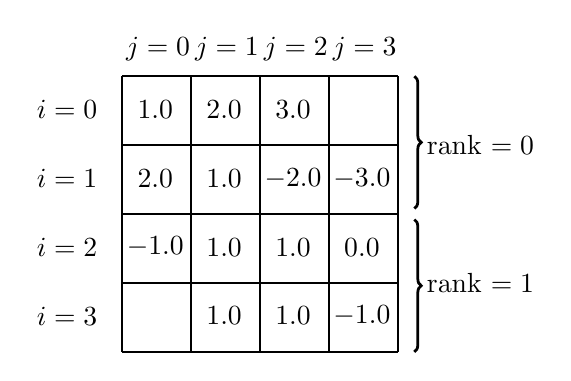
\begin{tikzpicture}[scale=3.5]
  \pgfmathsetmacro\fourth{1.0/4.0}
  \pgfmathsetmacro\xoff{0.12}
  \pgfmathsetmacro\yoff{0.12}
  \draw[xstep=\fourth,ystep=\fourth,black,thick] (0.0,0.0) grid (1.0,1.0);

  \node at (-0.2, 1.0-\yoff) {$i=0$};
  \node at (-0.2,0.75-\yoff) {$i=1$};
  \node at (-0.2, 0.5-\yoff) {$i=2$};
  \node at (-0.2,0.25-\yoff) {$i=3$};

  \node at ( 1.0-\xoff, 1.1) {$j=3$};
  \node at (0.75-\xoff, 1.1) {$j=2$};
  \node at ( 0.5-\xoff, 1.1) {$j=1$};
  \node at (0.25-\xoff, 1.1) {$j=0$};

  \node at (\xoff,1.0-\yoff) {$1.0$};
  \node at (0.25+\xoff,1.0-\yoff) {$2.0$};
  \node at (0.5+\xoff,1.0-\yoff) {$3.0$};
  \node at (0.75+\xoff,1.0-\yoff) {};

  \node at (\xoff,0.75-\yoff) {$2.0$};
  \node at (0.25+\xoff,0.75-\yoff) {$1.0$};
  \node at (0.5+\xoff,0.75-\yoff) {$-2.0$};
  \node at (0.75+\xoff,0.75-\yoff) {$-3.0$};

  \node at (\xoff,0.5-\yoff) {$-1.0$};
  \node at (0.25+\xoff,0.5-\yoff) {$1.0$};
  \node at (0.5+\xoff,0.5-\yoff) {$1.0$};
  \node at (0.75+\xoff,0.5-\yoff) {$0.0$};

  \node at (\xoff,0.25-\yoff) {};
  \node at (0.25+\xoff,0.25-\yoff) {$1.0$};
  \node at (0.5+\xoff,0.25-\yoff) {$1.0$};
  \node at (0.75+\xoff,0.25-\yoff) {$-1.0$};

  \draw[decoration={brace,mirror,raise=5pt},decorate,line width=1pt] (1.01,0.52) -- (1.01,1.0);
  \node at (1.3,0.752) {rank $=0$};
  \draw[decoration={brace,mirror,raise=5pt},decorate,line width=1pt] (1.01,0.0) -- (1.01,0.48);
  \node at (1.3,0.251) {rank $=1$};
\end{tikzpicture}
\bigskip
\caption{A parallel \pMat layout on two processes.  Blank entries are not allocated.}
\label{fig:mpitwomatlayout}
\end{marginfigure}

If the above lines appeared in \texttt{mycode.c}, and if it were run
\begin{cline}
$ mpiexec -n 2 ./mycode
\end{cline}
%$
then the layout would be as in Figure \ref{fig:mpitwomatlayout}.  \PETSc can show us the entries in the \pMat in different formats at runtime:
\begin{cline}
$ ./mycode -mat_view
Mat Object: 1 MPI processes
  type: seqaij
row 0: (0, 1)  (1, 2)  (2, 3)
row 1: (0, 2)  (1, 1)  (2, -2)  (3, -3)
row 2: (0, -1)  (1, 1)  (2, 1)  (3, 0)
row 3: (1, 1)  (2, 1)  (3, -1)
$ ./mycode -mat_view ::ascii_dense
Mat Object: 1 MPI processes
  type: seqaij
 1.00000e+00  2.00000e+00  3.00000e+00  0.00000e+00
 2.00000e+00  1.00000e+00  -2.00000e+00  -3.00000e+00
 -1.00000e+00  1.00000e+00  1.00000e+00  0.00000e+00
 0.00000e+00  1.00000e+00  1.00000e+00  -1.00000e+00
\end{cline}
The first view shows the compressed sparse storage, with values as pairs with column index and value.  The second view is a traditional (``dense'') display where all zero values are shown, whether allocated or not.  Other possibilities for outputting a \pMat, not shown, include ``\texttt{-mat\_view ::ascii\_matlab},'' which dumps in Matlab's text format, and ``\texttt{-mat\_view binary -viewer\_binary\_filename a.dat}'' which saves to file \texttt{a.dat} in \PETSc's scalable binary format.  In any case, \texttt{-mat\_view} output is activated by the \texttt{MatAssemblyBegin/End()} calls.

In these cases the matrix was stored in \emph{serial} compressed sparse row format, the \texttt{MATSEQAIJ} type, because of the one-process run.  If the code is run in parallel, i.e.~by \texttt{mpiexec -n N ./mycode}, then \texttt{-mat\_view}  reports \texttt{type:~mpiaij} corresponding to \pMat type \texttt{MATMPIAIJ}, the ``parallel compressed sparse row storage'' described above.


\section{Numerical linear algebra: residual, iterations, preconditioning}

Direct methods like Gauss elimination \citep{TrefethenBau} are one way to solve a linear system.  The most powerful methods for our later PDE-solving uses, however, are iterative.  They use the \emph{residual} of some approximation of the solution to the linear system.

By definition, the residual of $\bu_0$ in linear system \eqref{introsystem} is the vector
\begin{equation}
\br_0 = \bb - A \bu_0. \label{residualdefn}
\end{equation}
Evaluating the residual for a known vector $\bu_0$ requires only applying $A$ to it, an $O(N^2)$ operation at worst.  Because most discretization schemes for PDEs generate matrices $A$ that are \emph{sparse}, with many more zero entries than nonzeros, and because often the number of nonzeros per row is small and independent of $N$, the operation $A\bu_0$ and thus the evaluation of the residual can usually be done in $O(N)$ operations.

The \emph{Richardson iteration},\sidenote{Also called \emph{simple iteration} \citep{Greenbaum1997}.} simply adds a multiple $\omega$ of the last residual at each step,
\begin{equation}
\bu_{k+1} = \bu_k + \omega (\bb - A \bu_k).  \label{introrichardson}
\end{equation}
If significantly fewer than $O(N^2)$ steps were needed to make $\bu_k$ an adequate approximation of the exact solution $\bu$, then the Richardson iteration could improve on Gauss elimination.  On the other hand, the Richardson iteration may not converge, as in the next Example.

\medskip\noindent\hrulefill
\begin{example} Consider the linear system
\begin{equation}
A \bu
= \begin{bmatrix}
10 & -1 \\ -1 & 1
\end{bmatrix}
\begin{bmatrix} u_1 \\ u_2 \end{bmatrix}
= \begin{bmatrix} 8 \\ 1 \end{bmatrix}
= \bb
 \label{introexample}
\end{equation}
which has solution $\bu = [1\,\, 2]^\top$.  If we start with estimate $\bu_0 = [0\,\, 0]^\top$ then the $\omega=1$ Richardson iteration \eqref{introrichardson} gives a sequence of vectors % see ../matlab/richardsonex.m
\begin{equation}
\rvect{0}{0}{0}, \rvect{1}{8}{1}, \rvect{2}{-63}{9}, \rvect{3}{584}{-62}, \dots
\end{equation}
This sequence is not heading toward the solution.
\end{example}
\noindent\hrulefill

\medskip
If we rewrite \eqref{introrichardson} as
\begin{equation}
\bu_{k+1} = (I - \omega A) \bu_k + \omega \bb  \label{introrewriterichardson}
\end{equation}
then it is easy to believe that the ``size'' of the matrix $I-\omega A$ will determine whether $\lim_{k\to\infty} \bu_k$ exists.

To make this precise we recall important definitions.  A complex number\sidenote{Though $B$ is real, $\lambda$ may indeed be complex, but if $\lambda$ is an eigenvalue of a real matrix $B$ then so is $\bar\lambda$.} $\lambda \in \CC$ is an \emph{eigenvalue} of a square matrix $B\in\RR^{N\times N}$ if there is a nonzero vector $\bv\in\CC^N$ so that $B \bv = \lambda \bv$.  The set of all eigenvalues of $B$ is the \emph{spectrum} $\sigma(B)$ of $B$.  The \emph{spectral radius} $\rho(B)$ is the maximum magnitude of the eigenvalues of $B$.  The \emph{singular values} are the square roots of the eigenvalues of the matrix $B^*B$, a symmetric and positive-definite matrix with nonnegative eigenvalues.  Singular values are geometrically-defined as the lengths of semi-axes of the (hyper-)ellipsoid in $\RR^N$ that results from applying $B$ to all vectors in the unit ball of $\RR^N$ \citep{TrefethenBau}.

Properties of a matrix described in terms of its eigenvalues or singular values are generically called ``spectral properties.''  For example, $\|B\|_2$ is the largest singular value of $B$ and $\|B^{-1}\|_2$ is the inverse of the smallest singular value of $B$, so these are spectral properties.  The 2-norm condition number $\kappa(B)=\|B\|_2/\|B^{-1}\|_2$ is thus also a spectral property; it is visualized as the eccentricity of the ellipsoid above.

It is an easy exercise to show that the Richardson iteration \eqref{introrichardson} or \eqref{introrewriterichardson} will converge if and only if all the eigenvalues of $B=I-\omega A$ are inside the unit circle:
\begin{equation}
\text{\eqref{introrichardson} converges if and only if } \rho(I-\omega A) < 1. \label{introconvergethm}
\end{equation}
One can also show that $\rho(B) \le \|B\|$ using any induced matrix norm, so \eqref{introrichardson} converges if $\|I-\omega A\| < 1$.

Considering spectral properties brings us to an important general point about linear systems.  Namely, that there are many systems which are equivalent to \eqref{introsystem}.  In fact, if $M\in\RR^{N\times N}$ is an invertible matrix then the systems
\begin{equation}
(M^{-1} A) \bu = M^{-1} \bb \label{introleftpre}
\end{equation}
and
\begin{equation}
(A M^{-1}) (M\bu) = \bb \label{introrightpre}
\end{equation}
have the same solution(s) $\bu$ as \eqref{introsystem}.  However, matrices $M^{-1} A$ or $A M^{-1}$ generally have different eigenvalues, condition numbers, and so on---different spectral properties---from $A$.  While the accuracy of the approximate solution $\bu$ cannot be improved beyond the $\kappa(A) \eps$ level, as fact i) on page \pageref{limittoaccuracy} cannot be overcome, methods can take advantage of the better spectral properties of $M^{-1} A$ or $A M^{-1}$, relative to $A$, to generate approximations to $\bu$ more quickly.  This idea is effective if $M^{-1}$ is easy to apply, in the sense that substantially fewer operations are needed to solve the system $M\bv=\bc$ than the original system $A\bu=\bb$.

Systems \eqref{introleftpre} and \eqref{introrightpre} are referred to as \emph{preconditioned} versions of \eqref{introsystem}, with \eqref{introleftpre} called \emph{left preconditioning} and \eqref{introrightpre} called \emph{right-preconditioning}.  The next example shows how preconditioning can make the Richardson iteration converge.  In this case the diagonal of $A$ is used as $M$, so it is an example of \emph{Jacobi preconditioning}.

\medskip\noindent\hrulefill
\begin{examplecont}  Suppose we extract the diagonal of $A$ from  \eqref{introexample}:
\begin{equation}
M = \begin{bmatrix}
10 & 0 \\ 0 & 1
\end{bmatrix}.  \label{introM}
\end{equation}
Being diagonal, $M$ is easy to invert and apply.  The preconditioned Richardson iteration using $M$, namely
\begin{equation}
\bu_{k+1} = \bu_k + \omega (M^{-1} \bb - M^{-1} A \bu_k),  \label{introprerichardson}
\end{equation}
is better behaved.  With $\bu_0 = [0\,\, 0]^*$ and $\omega=1$ again we get this sequence from \eqref{introprerichardson}:
\begin{equation}
\rvect{0}{0}{0}, \rvect{1}{0.8}{1.0}, \rvect{2}{0.9}{1.8}, \rvect{3}{0.98}{1.90}, \dots
\end{equation}
This sequence is apparently going to $\bu = [1\,\, 2]^*$.  The explanation is not hard to see; compare
\begin{equation}
\rho(I-A) = -9.1 \quad \text{and} \quad \rho(I-M^{-1} A) = 0.32,
\end{equation}
which illustrates convergence claim \eqref{introconvergethm}.
\end{examplecont}
\noindent\hrulefill

\medskip
Let us note one more idea associated to the residual.  Intuitively speaking, a vector norm of a residual, for example $\|\br_0\| = \|\bb - A \bu_0\|$, measures how ``wrong'' is $\bu_0$ as an approximation to $\bu=A^{-1}\bb$, but this idea is incomplete in two senses.  First, we surely would want the norm of the \emph{error} itself, i.e.
\begin{equation}
\be_0 = \bu_0 - \bu \label{errordefn}
\end{equation}
as an authentic measure of how wrong $\bu_0$ is.  However, given $\bu_0$, by \eqref{errordefn} exact knowledge of the error $\be_0$ is equivalent to exact knowledge of the solution $\bu$ itself.  Only bounds on $\|\be_0\|$ might be reasonably be expected, even though we can compute the full residual vector $\br_0 = \bb - A \bu_0$ at will.  Secondly, errors are most meaningful if they are relative.  For instance, knowing ``$\|\be_0\|\le 10^{-6}$'' does not tell us that $\bu_0$ is an accurate solution to the system $A \bu = \bb$ if $\|A^{-1}\|=1$ and $\|\bb\|= 10^{-6}$, in which case we know in advance that $\|\bu\|\le 10^{-6}$.

These ideas relate to the conditioning of $A$.  Indeed, the connection between the relative norm we \emph{can} compute, namely $\|\br_0\|/\|\bb\|$, and the relative norm we \emph{want} is well-known:
\begin{equation}
\kappa(A)^{-1} \frac{\|\br_0\|}{\|\bb\|} \le \frac{\|\be_0\|}{\|\bu\|} \le \kappa(A) \frac{\|\br_0\|}{\|\bb\|}, \label{relativenormbounds}
\end{equation}
where $\kappa(A) = \|A\| \|A^{-1}\|$ is the condition number in the induced norm.  Proving \eqref{relativenormbounds} is an easy exercise with norms.


\section{Numerical linear algebra: Krylov space methods}

The most powerful iterative methods for solving system \eqref{introsystem} generate optimal, in various senses, estimates $\bu_k$ which are linear combinations of vectors $\bz,A\bz,A^2\bz,\dots,A^{k-1}\bz$ where $\bz$ is a fixed vector; often $\bz=\bb$.  These methods are collectively called \emph{Krylov space methods} because the span of such vectors is a \emph{Krylov space}.  Examples include the Richardson iteration, conjugate gradient (CG), and minimum residual methods (MINRES or GMRES).\sidenote{We will address these method in this and the next chapter, but see \citet{Greenbaum1997} or \citet{Saad2003} for details and algorithms.}  The effectiveness of a given Krylov method on a given system depends on the eigenvalues or singular values of the matrix $A$, i.e.~on its spectral properties.  Many Krylov space methods are built into and fully-supported by \PETSc, and we will use them in all later Chapters.

To be concrete, a Krylov space is defined as
\begin{equation}
    \mathcal{K}_n(A,\bb) = \operatorname{span}\{\bb,A\bb,A^2\bb,\dots,A^{n-1}\bb\}, \label{eq:li:krylovdefn}
\end{equation}
but we give the abbreviated name ``$\mathcal{K}_n$'' when the context is clear.  Suppose $\tilde\bu \in \mathcal{K}_n$.  Then
    $$\tilde\bu = c_0 \bb + c_1 A \bb + c_2 A^2 \bb + \dots + c_{n-1} A^{n-1} \bb$$
for some coefficients $c_j$, or equivalently
    $$\tilde\bu = p_{n-1}(A) \bb$$
for the $n-1$ degree polynomial $p_{n-1}(x) = c_0 + c_1 x + \dots + c_{n-1} x^{n-1}$ applied to $A$.

Thus if we want $\tilde\bu$ to approximate $\bu$, the solution to \eqref{introsystem}, then we want to find a polynomial $p_{n-1}$ so that
\begin{equation}
    p_{n-1}(A) \approx A^{-1},  \label{krylovgoal}
\end{equation}
at least in the action of applying $p_{n-1}(A)$ to $\bb$.  Krylov space methods do this.

One can prove that if $p_{n-1}(z)$ is close to $1/z$ on the finite set of eigenvalues of $A$, i.e.~on the spectrum $\sigma(A)$ in the complex plane, then \eqref{krylovgoal} follows.  Thus, whether $p_{n-1}$ is a ``good'' polynomial for approximately inverting $A$ is a spectral question about $A$.  The construction of a ``good'' $p_{n-1}$ would be only a question of approximation theory in the complex plane if only the spectrum $\sigma(A)$ were known, but in fact that is asking too much!  We know $A$ through its entries or action on vectors, and we might have general spectral information about $A$ through the context in which it was generated,\sidenote{As the discretization of a PDE with known spectral properties, for example.} but accurately computing its full spectrum $\sigma(A)$ is at least as difficult as solving a linear system $A\bu=\bb$.

For an example in which polynomial generation from a Krylov method can be seen, consider again the Richardson iteration \eqref{introrichardson} with $\omega=1$, namely $\bu_{k+1} = \bu_k + (\bb - A \bu_k)$.  A straightforward calculation starting with $\bu_0=\bb$ shows
\begin{equation}
	\bu_k = q_k(A) \bb \quad \text{with} \quad q_{k+1}(x) = 1 + (1-x) q_k(x)  \label{richpolys}
\end{equation}
and $q_0(x)=1$.
%see richpolyplot.py for formulas
Figure \ref{fig:richpolyplot} shows these polynomials.  It is easy to check that $q_k(x) \to 1/x$ for $x\in (0,2)$, and the Figure suggests it too.  On the other hand, \eqref{introconvergethm} says $q_k(A) \bb \to A^{-1} \bb$ if the spectral condition $\rho(I-A)<1$ holds.  This condition says exactly that all eigenvalues of $A$ must be within distance one of $1+0i$ in the complex plane, and thus that all real eigenvalues of $A$ must be in $(0,2)$.

\begin{figure}
\bigskip
\includegraphics[width=0.8\textwidth]{richpolyplot}
\caption{The $\omega=1$ case of the Richardson iteration \eqref{introrichardson} approximates $\bu=A^{-1}\bb$ by $\bu_k=q_k(A)\bb$.  These polynomials $q_k(x)$ approximate $1/x$ on the interval $(0,2)$.}
\label{fig:richpolyplot}
\end{figure}

Though the Richardson iteration generates $\bu_k$ which are from a Krylov space, and thus from polynomials in $A$ applied to $\bb$, they are by no means the best such approximations.  We now give a ``gloss'' of two other well-known Krylov methods.  They generated the same kind of polynomial approximations, but for polynomials $p_n$ which minimize vector norms over a Krylov space.

\newcommand{\Pnone}{\mathcal{P}_n^1}
\newcommand{\Kone}[2]{\mathcal{K}_{#1}^1(#2)}
Define $\Pnone$ to be the set of all real polynomials $p$ of degree $n$ such that $p(0)=1$.  For a real square matrix $A \in \RR^{N\times N}$ and $\bv\in\RR^N$, define the affine space (set)
	$$\Kone{n}{A,\bv} = \bv + \Span\{A\bv,A^2\bv,\dots\,A^{n-1}\bv\}.$$
In these terms, Figure \ref{tab:krylovcompare} compares three of the best-known Krylov methods, namely the Richardson iteration \eqref{introrichardson}, conjugate gradients (CG), and generalized minimum residuals (GMRES).  

For CG and GMRES as algorithms, see \citet{Greenbaum1997} or \citet{Saad2003}.  Regarding GMRES, note that in practice it uses ``restarts'' to avoid filling memory with its internal representation of the Krylov space, and this action stops it from being a ``pure'' Krylov method (i.e.~one based on a fixed initial vector to form the Krylov space).  The \PETSc default is to restart after 30 iterations, so GMRES uses $\sim 30N$ memory locations on an $N$-dimensional problem, compared to $3N$ for CG and $2N$ for Richardson.

The classical \emph{Jacobi} and \emph{Gauss-Seidel iterative methods} \citep{Greenbaum1997} are not Krylov space methods as they stand.  They involve extracting parts of (entries of) $A$, as a matrix, which can not be done by operations $A^k\bv$.  These classical iterations can, however, be regarded as preconditioned forms of the Richardson iteration \citep{Greenbaum1997}; see the Exercises.

\newcommand{\mpwide}{28mm}
\bigskip
\begin{figure}[h]
\small
\begin{tabular}{llll} \vspace{5mm}
\emph{NAME}\hspace{0.5in} & Richardson & CG & GMRES \\ \vspace{5mm}
\emph{SYMMETRY} & any & \begin{minipage}[l]{\mpwide}symmetric positive-definite\end{minipage} & any \\ \vspace{5mm}
\emph{OPTIMALITY} & none & \begin{minipage}[l]{25mm}$\be_k$ minimizes $f(\bv){=}\left<\bv,A\bv\right>$ over $\bv{\in}\Kone{k}{A,\be_0}$\end{minipage} & \begin{minipage}[l]{\mpwide}$\br_k$ minimizes $f(\bv){=}\|\bv\|_2$ over $\bv{\in}\Kone{k}{A,\bb}$\end{minipage} \\ \vspace{5mm}
\begin{minipage}[l]{21mm}\emph{SPECTRAL} \emph{CONDITION}\end{minipage} & $\rho(I-\omega A) \ll 1$ & \begin{minipage}[l]{\mpwide}exist $p_n{\in}\Pnone$ small on $\sigma(A){\subset}(0,\infty)$\end{minipage} & \begin{minipage}[l]{\mpwide}exist $p_n{\in}\Pnone$ small on $\sigma(A){\subset}\CC$\end{minipage}
\end{tabular}
\caption{Comparison of three well-known Krylov methods for the problem $A\bu=\bb$.  ``Symmetry'' refers to the required properties of $A$ so as to apply the method.  ``Spectral condition'' is an informal statement of the spectral properties of $A$ which will lead to rapid convergence.  Here $\br_k=\bb-A\bu_k$ and $\be_k=\bu_k-\bu$.} \label{tab:krylovcompare}
\end{figure}

We get access to the many Krylov methods implemented in \PETSc any time we create a \pKSP object.  Which method is used can be controlled at runtime, as long as we call the \texttt{KSPSetFromOptions()} method (below), and runtime experimentation is always appropriate.  For the Poisson problem in Chapter \ref{chap:structured}, for example, we will see that preconditioned CG is very effective, but in later Chapters we will put the most emphasis on the preconditioning stage.  We will see that multigrid preconditioning is extraordinarily effective on the Poisson problem (Chapter \ref{chap:multigrid}).  And we will return to Krylov space methods repeatedly in later Chapters.

Our brief introduction of iterative linear algebra is hardly adequate.  But we need now to return to \PETSc codes and solve linear systems.  In the upcoming material the reader can initially treat \PETSc's \pKSP linear solver object as a black box, but then explore how it works through runtime options.


\section{A small linear system}

We already know how to create, fill, and destroy \pVec and \pMat objects.  The next code, \texttt{vecmatksp.c} in Figure \ref{code:vecmatksp}, does these steps.  It also uses a \pKSP object to actually solve the linear system.  The specific Krylov iteration, inside the \pKSP, is chosen at runtime.  The expected \texttt{Create/SetFromOptions/Destroy} sequence applies to a \pKSP.

There are, however, two additional commands, or their equivalents, needed even for the simplest examples.  First we need to tell \pKSP about the matrix via the command
\begin{code}
KSPSetOperators(ksp,A,A);
\end{code}
Then the system is actually solved by
\begin{code}
KSPSolve(ksp,b,x);
\end{code}
which also supplies the right-hand side of the system (i.e.~an allocated and assembled \pVec \texttt{b}) and space for the solution (an allocated \pVec \texttt{x}).

Why do we list \texttt{A} twice in calling \texttt{KSPSetOperators()}?  Recall the linear system $A\bx=\bb$ is equivalent to $M^{-1} A \bx = M^{-1} \bb$ (left preconditioning).  At runtime we generally choose a preconditioning method which builds $M^{-1}$ from $A$ or from an approximation of $A$.  For example, \emph{incomplete LU} factorization of $A$ can be used in generating $M^{-1}$, or $M$ could be the diagonal of $A$ (as in the example above).  The second matrix argument to \texttt{KSPSetOperators()} is the \pMat from which $M^{-1}$ is built.  Note we do not supply $M$ itself; that would block easy choice among preconditioners at runtime.\sidenote{And require the user to write extra code.}  Instead we supply ``material'' from which the preconditioning action $M^{-1}$ is built.  The most common such material is $A$ itself.

After calling \texttt{KSPSolve()} we display the solution \pVec by calling \texttt{VecView()}.  This and everything else about the code in Figure \ref{code:vecmatksp} should now be self-explanatory.  So let's compile and run it:
\begin{cline}
$ cd c/ch2/
$ make vecmatksp
$ ./vecmatksp
Vec Object: 1 MPI processes
  type: seq
1
0
2
-1
\end{cline}
%$
This solves the system and gives us $\bx$.  But what happened and how to control it?

\vfill
\clearpage
\inputwhole{../c/ch2/vecmatksp.c}{\texttt{c/ch2/vecmatksp.c}}{Solve a small linear system.}{code:vecmatksp}


\section{Revealing solvers at runtime}

To start to see what happened when we ran \texttt{./vecmatksp} above, we could start by viewing the \pVec and \pMat objects.  In fact, the result of doing
\begin{cline}
$ ./vecmatksp -vec_view -mat_view
\end{cline}
%$
should be completely as expected, and thus it is not shown.  This output tells us nothing about the solution process, however, and it gives no hints on alternative ways of solving the equations.

Here is a key idea which cannot be over-emphasized:
\begin{quote}
\emph{learning \PETSc requires viewing \emph{solver} objects at runtime.}
\end{quote}
Here we try \texttt{-ksp\_view}; the output is slightly-clipped for clarity:
\begin{cline}
$ ./vecmatksp -ksp_view
KSP Object: 1 MPI processes
  type: gmres
    GMRES: restart=30, using Classical (unmodified) Gram-Schmidt ...
    GMRES: happy breakdown tolerance 1e-30
  maximum iterations=10000, initial guess is zero
  tolerances:  relative=1e-05, absolute=1e-50, divergence=10000
  left preconditioning
  using PRECONDITIONED norm type for convergence test
PC Object: 1 MPI processes
  type: ilu
    ILU: out-of-place factorization
    0 levels of fill
    tolerance for zero pivot 2.22045e-14
    matrix ordering: natural
    factor fill ratio given 1, needed 1
      ...
  linear system matrix = precond matrix:
  Mat Object:   1 MPI processes
    type: seqaij
    rows=4, cols=4
    total: nonzeros=16, allocated nonzeros=20
    total number of mallocs used during MatSetValues calls =0
      using I-node routines: found 1 nodes, limit used is 5
Vec Object: 1 MPI processes
  type: seq
1
0
2
-1
\end{cline}
%$
Here is some of what we learn:
\begin{itemize}
\item The default \pKSP solver is GMRES.  This is \texttt{-ksp\_type gmres} as a command-line option.
\item As noted, GMRES restarts after a number of iterations so as to limit memory usage.  The default is \texttt{-ksp\_gmres\_restart 30} as an option.
\item The default convergence tolerances for the \pKSP are \texttt{-ksp\_rtol 1.0e-5} and \texttt{-ksp\_atol 1.0e-50}.  In particular, \pKSP iterations stop when the residual norm has been reduced by $10^5$.
\item Inside the \pKSP is a \pPC preconditioner object.  We did not have to ask for one when writing the code, as every \pKSP has a \pPC.
\item The default \pPC is left preconditioning with ILU, i.e.~incomplete LU factorization, which is \texttt{-pc\_type ilu} as a runtime option.\sidenote{We will see in a moment that this is the \emph{serial} default \pPC, and there is more going on in parallel.}
\item The \pPC object has a copy of $A$ (``\texttt{Mat Object}''), because it was supplied as the second argument to \texttt{KSPSetOperators()} above.
\item The preconditioner has ``\texttt{0 levels of fill}'',\sidenote{Thus it is usually called ``ILU($0$)''.} so it uses no more memory than is used by the copy of $A$ which is supplied to \texttt{KSPSetOperators()}.
\end{itemize}
Of course, we get the solution $\bx$ too.

While option \texttt{-ksp\_view} tells us what the solver \emph{is}, option \texttt{-ksp\_monitor} shows what it \emph{does}.  In this case, the \pKSP iteration is short:
\begin{cline}
$ ./vecmatksp -ksp_monitor
  0 KSP Residual norm 2.449489742783e+00
  1 KSP Residual norm 1.520235486122e-15
Vec Object: 1 MPI processes
...
\end{cline}
%$
The reason that the residual drops to nearly zero in one iteration is that GMRES sees a preconditioned system with an identity matrix in this case.  That is, $P^{-1} A = I$ because the ILU operation on this particular $A$ is actually a full LU factorization.  Our $A$ is banded and ``dense enough'' so that the LU factorization requires no fill-in.

For a small system like this a direct solve also works fine.  To see how to do it, first do
\begin{cline}
$ ./vecmatksp -help | grep ksp_type
  -ksp_type <gmres>: Krylov method (one of) cg ... preonly ... (KSPSetType)
$ ./vecmatksp -help | grep pc_type
  -pc_type <ilu>: Preconditioner (one of) none jacobi ... lu ... (PCSetType)
\end{cline}
to see the many solver and preconditioner options.  One of the preconditioners is ``\texttt{lu}'', suggesting a direct solve.  In this case we \emph{do not} want iterations, and one of the \pKSP options is ``\texttt{preonly}''.  Thus the direct solver combination we want is
\begin{cline}
$ ./vecmatksp -ksp_type preonly -pc_type lu
\end{cline}
%$
The reader should check that the output of \texttt{-ksp\_view} is as intended.

When solving on multiple processors, using ILU($0$) as the default preconditioner makes no sense.  This is because, even when fill-in is avoided, the LU factorization algorithm would involve a great deal of interprocessor communication.  However, there are blocks along the diagonal of the system matrix $A$ which are entirely owned by a single processor.  The ILU($0$) method can be applied to these, and the result treated as an approximation $P^{-1}\approx A^{-1}$.  That is, the blocks along the diagonal can be approximately inverted by ILU($0$), and the result treated as a block-diagonal (i.e.~block-Jacobi) preconditioner.

The default \PETSc \pKSP settings \emph{in parallel} correspond to options
\begin{quote}
\texttt{-ksp\_type gmres -pc\_type bjacobi -sub\_pc\_type ilu}
\end{quote}
This is what they do:
\begin{itemize}
\item The default \pKSP remains GMRES with restart 30.
\item The default \pPC is now \texttt{bjacobi}, i.e.~application of approximate diagonal-block inverses as $M^{-1}$.
\item Inside the \pPC is a \texttt{sub\_pc} object, also a \pPC, which is ILU($0$),\sidenote{There is even a \texttt{sub\_ksp} object, but it is \texttt{preonly}.  So let's just ignore that complication for now.} and this generates the approximate diagonal-block inverses.
\end{itemize}
The reader can confirm this understanding of the situation by running
\begin{cline}
mpiexec -n 2 ./vecmatksp -ksp_view
\end{cline}

But surely that's enough runtime options for now.  There will be more, especially in later chapters when we solve PDEs.


\section{A sparse system of arbitrary size}

We have seen \PETSc code to set up and solve linear systems, but there is more to say.  The next example \texttt{tri.c}, split into Figures \ref{code:tripartone} and \ref{code:triparttwo}, introduces these additional concepts and their associated function calls:
\begin{enumerate}
\item Creating an option, so that the size of the linear system can be controlled at runtime, by using \texttt{PetscOptionsXXX()} calls.
\item Using \texttt{VecDuplicate()} for allocation.
\item Assembling a system of arbitrary size across an arbitrary number of processes, using \texttt{MatGetOwnershipRange()} to only set locally-owned rows.
\item Using \texttt{VecAXPY()}, \texttt{VecNorm()}, and \texttt{PetscPrintf()} to compute and display the error in a case where the exact solution is known.
\end{enumerate}

\vfill
\newpage
\cinputpartnostrip{tri.c}{c/ch2/}{Set up \pVec and \pMat objects for a tridiagonal system.}{I}{//STARTSETUP}{//ENDSETUP}{code:tripartone}

First build and run the code with options that show what it is does by default:
\begin{cline}
$ make tri
$ ./tri -ksp_monitor -a_mat_view ::ascii_dense
Mat Object:(a_) 1 MPI processes
  type: seqaij
  3.00000e+00  -1.00000e+00   0.00000e+00   0.00000e+00 
 -1.00000e+00   3.00000e+00  -1.00000e+00   0.00000e+00 
  0.00000e+00  -1.00000e+00   3.00000e+00  -1.00000e+00 
  0.00000e+00   0.00000e+00  -1.00000e+00   3.00000e+00 
  0 KSP Residual norm 3.302822756884e+00 
  1 KSP Residual norm 5.519370044893e-16 
error for m = 4 system is |x-xexact|_2 = 5.1e-16
\end{cline}

To get started on the new concepts shown in Figure \ref{code:tripartone}, notice that methods \texttt{PetscOptionsBegin()} and \texttt{PetscOptionsEnd()} bracket the call to \texttt{PetscOptionsInt()}.  We set an option prefix ``\texttt{-tri\_...}'' so that the new option we create is distinguished from the many built-in \PETSc options that start with \texttt{-ksp\_...} or \texttt{-vec\_...} or whatever.  Our use of \texttt{PetscOptionsInt()} creates an option \texttt{-tri\_m} which allows the user to set the variable \texttt{m}, and to leave the default \texttt{m}$=4$ unaltered if the option is not set.

To see the option and its default value in \texttt{-help} output do
\begin{cline}
$ ./tri -help | grep tri_
Solve a tridiagonal system of arbitrary size.  Option prefix = tri_.
  -tri_m <4>: dimension of linear system (None)
\end{cline}
Here, for instance, we reset the system size to be small and we view the matrix:
\begin{cline}
$ ./tri -tri_m 2 -a_mat_view
Mat Object:(a_) 1 MPI processes
  type: seqaij
row 0: (0, 3)  (1, -1) 
row 1: (0, -1)  (1, 3) 
error for m = 2 system is |x-xexact|_2 = 8.0e-16
\end{cline}
%$

After setting up the new option, next in \texttt{tri.c} the numerical solution \pVec \texttt{x} is created just as we did in the last example \texttt{vecmatksp.c} (Figure \ref{code:vecmatksp}).  But now we also want to create \pVecs \texttt{b} and \texttt{xexact}; the former is the right-hand side of the linear system and the latter holds the exact solution to the linear system so that we can evaluate the error in the numerical solution.  Though at this stage we have not filled any entries of \texttt{x}, we can save repetitive function calls to \texttt{VecCreate/SetSizes/SetFromOptions()} when creating these additional \pVecs.  That is, because they have the same properties and parallel layout we can use \texttt{VecDuplicate()} to allocate \pVecs just like \texttt{x}.\sidenote{There is a different method for copying the contents of \pVecs, namely \texttt{VecCopy()}.  It requires that the two \pVecs are already allocated and have the same layout.}

Next we assemble the matrix $A$.  This is a boring tridiagonal matrix with $3$ on the diagonal and $-1$ in the super- and sub-diagonals.  Though boring, we want to assemble it efficiently in parallel, something that will be important when solving 2D and 3D PDEs in later chapters.  However, only when \texttt{tri.c} is run do we know how many processes are in use.  A key method for efficient matrix assembly in parallel is the method \texttt{MatGetOwnershipRange()} which tells our program, as it is running on a particular process (rank), what rows it owns locally.  In the case of a many structured matrices like this one, we can avoid all interprocess communication by assembling exactly the rows we own.  As seen at the top of Figure \ref{code:triparttwo}, we call
\begin{quote}
\texttt{MatGetOwnershipRange(A,\&Istart,\&Iend)}
\end{quote}
to get the starting and ending row indices for the local process.  These are used as limits in a \texttt{for} loop over the locally own rows, wherein we call \texttt{MatSetValues()} to actually set the entries of $A$.  We call \texttt{MatAssemblyBegin/End()} to complete the assembly of $A$.

\cinputpartnostrip{tri.c}{c/ch2/}{Assemble and solve.}{II}{//ENDSETUP}{//ENDSOLVE}{code:triparttwo}

We need to assemble the right-hand side $\bb$ of the linear system.  But this is related to the question: how does one get the exact solution $\bx_{\text{exact}}$ to a linear system $A\bx_{\text{exact}} = \bb$?  The easiest way for demonstration purposes, as here, is to \emph{choose} $\bx_{\text{exact}}$ and then compute $\bb$ by multiplying by $A$.  Thus, we set (unimportant) values for \texttt{xexact}, and call \texttt{VecAssemblyBegin/End()} on it.  Then we compute \texttt{b} by calling \texttt{MatMult(A,xexact,b)}.

As in the earlier code, we set up  the \pKSP and then call \texttt{KSPSolve()} to approximately solve $A\bx = \bb$.  As the \pKSP is working we can see it reduce the $k$th-iteration residual norm $\|\bb-A\bx_k\|_2$ just by using option \texttt{-ksp\_monitor}.  In this case we also want to see that the actual error
	$$\|\bx - \bx_{\text{exact}}\|_2$$
is small when the \pKSP completes its work.  So, after getting \texttt{x} from \texttt{KSPSolve()} we compute the error with two commands,

\medskip
\begin{tabular}{lcrcl}
\text{\texttt{VecAXPY(x,-1.0,xexact)}}       & : & $\bx$                   & $\leftarrow$ & $-1\, \bx_{\text{exact}} + \bx$ \\
\text{\texttt{VecNorm(x,NORM\_2,\&errnorm)}} & : & \text{\texttt{errnorm}} & $\leftarrow$ & $\|\bx\|_2$.
\end{tabular}

\medskip
\noindent and then print \texttt{errnorm} by calling \texttt{PetscPrintf()}.


\section{A first look at performance}

The linear system assembled by \texttt{tri.c} is about as easy to solve as they get.   It is tridiagonal, symmetric, diagonally-dominant, and positive definite.\sidenote{See Exercise \ref{exer:computeeigs}.}  So \PETSc ought to be able to solve it quickly, almost all Krylov methods should apply, and parallelization ought to be effective.

\newcommand{\WORKSTATION}{\textsc{workstation}\xspace}
We can time a one-process solution:
\begin{cline}
$ time ./tri -tri_m 10000
error for m = 10000 system is |x-xexact|_2 = 8.0e-13
real 0.04
user 0.04
sys 0.00
\end{cline}
%$
\label{defineworkstation}
These times were taken on the author's 2012-era workstation with 16 GB memory and a single Intel Core i7-3820 4-core cpu running at 3.60GHz.  From now on we call this machine \WORKSTATION.

Only the ``\texttt{real}'' time above is worth considering.  From now on we will use an alias to get just this time:
\begin{cline}
$ alias timer='time -f "real %e"'
\end{cline}
%$

The above timing result of $.04$ seconds suggests that this $m=10^4$ dimension system is not yet big enough to be worth testing, so we experiment on what $m$ gives a linear system with noticeable solution time.  Here is a roll-your-own bash loop to time some bigger solves:
\begin{cline}
$ export SIZES="10000 100000 1000000 10000000"
$ for M in $SIZES; do timer ./tri -tri_m $M; done
error for m = 10000 system is |x-xexact|_2 = 8.0e-13
real 0.01
error for m = 100000 system is |x-xexact|_2 = 3.1e-12
real 0.07
error for m = 1000000 system is |x-xexact|_2 = 4.8e-11
real 0.32
error for m = 10000000 system is |x-xexact|_2 = 3.5e-10
real 2.39
\end{cline}
We see that the default \PETSc \pKSP and \pPC methods\sidenote{GMRES with ILU($0$) preconditioning.} solve a system of size $m=10^7$ (ten million) in a time of a few seconds on \WORKSTATION.  Will other methods and/or more processors speed up the solution of the linear system of this size?

We can try a direct solve (\texttt{-ksp\_type preonly -pc\_type lu}), the default serial solver (\texttt{-ksp\_type gmres -pc\_type ilu}), and the default parallel solver (\texttt{-ksp\_type gmres -pc\_type bjacobi -sub\_pc\_type ilu}).  We can turn off preconditioning (\texttt{-pc\_type none}) or switch from ILU($0$)-based preconditioning to Jacobi preconditioning (\texttt{-pc\_type jacobi}).

Thus, to generate Table \ref{tab:tritiming} below, we did 16 runs which looked like this:
\begin{cline}
$ timer mpiexec -n N ./tri -tri_m 20000000 -ksp_rtol 1.0e-10 -ksp_type KSP -pc_type PC
\end{cline}
%$
for $N=1$ and $N=4$, and several \pKSP/\pPC choices.  The tighter tolerance \texttt{-ksp\_rtol 1.0e-10} was added because a fair comparison of iterative and direct methods needs significant accuracy in the iterative ones.

\newcommand{\intime}[1]{\input{timing/tri/#1}}
\begin{table}
\texttt{
\begin{tabular}{llll}
\underline{KSP}\hspace{0.5in} & \underline{PC}\hspace{0.8in} & \underline{N=1 \textrm{time (s)}}\hspace{0.3in} & \underline{N=4 \textrm{time (s)}} \\
preonly    & lu          & \intime{preonly.lu.1}       &  \\
           & cholesky    & \intime{preonly.cholesky.1} &  \\
richardson & jacobi      & \intime{richardson.jacobi.1}& \intime{richardson.jacobi.4} \\
gmres      & none        & \intime{gmres.none.1}       & \intime{gmres.none.4} \\
           & jacobi      & \intime{gmres.jacobi.1}     & \intime{gmres.jacobi.4} \\
           & ilu         & \intime{gmres.ilu.1}        &  \\
           & bjacobi+ilu &                             & \intime{gmres.bjacobi.4} \\
cg         & none        & \intime{cg.none.1}          & \intime{cg.none.4} \\
           & jacobi      & \intime{cg.jacobi.1}        & \intime{cg.jacobi.4} \\
           & icc         & \intime{cg.icc.1}           &  \\
           & bjacobi+icc &                             & \intime{cg.bjacobi.4} \\
\end{tabular}
}
\caption{Times for \texttt{tri.c} to solve systems of dimension $m=2\times 10^7$.  In this case the matrix is \emph{tridiagonal}, \emph{symmetric}, \emph{diagonally-dominant}, and \emph{positive definite}.  All runs were on \WORKSTATION (see page \pageref{defineworkstation}).} \label{tab:tritiming}
\end{table}

This Table deserves discussion:
\begin{itemize}
\item Entries ``\texttt{bjacobi+ilu}'' and ``\texttt{bjacobi+icc}'' correspond to options \texttt{-pc\_type bjacobi -sub\_pc\_type ilu} and \texttt{-pc\_type bjacobi -sub\_pc\_type icc}, respectively.  As already noted, the first of these is the parallel default.\sidenote{This example suggests it is a reasonable choice for the default!}
\item Counting floating point operations shows the leading-order work for Cholesky is $m^3/3$ while for LU it is $2 m^3/3$ \citep{TrefethenBau}.  This is reflected in the direct-solve results using \texttt{-ksp\_type preonly}.  A diagonally-dominant tridiagonal problem is very well-behaved for direct methods because no fill-in or pivoting occurs when they are applied, but we should not assume that a generic $10^7$ dimension systems are good candidates for direct solves.
\item Cholesky and CG methods apply to symmetric positive-definite matrices only.  These are \pKSP method \texttt{cg} and \pPC methods \texttt{cholesky} and \texttt{icc} (incomplete-Cholesky, also denoted ``IC($0$)'').  We see some benefit to using CG on one-process runs, compared to the general (non-symmetric) method GMRES, but the matrix generated by \texttt{tri.c} is so well-behaved that both of these iterations work well.
\item There is some speed-up from $N=1$ to $N=4$ processes on this single node 4-core \WORKSTATION.  The two (or slightly more) times speed-up is relatively uniform across methods.  But apparently using four cores does not guarantee anywhere near four-times speed-up.
\end{itemize}

In future Chapters, ``real'' linear and non-linear systems will be generated by discretizing PDEs.  Then we will create timing tables like Table \ref{tab:tritiming}, and re-consider the results.

\begin{marginfigure}
\bigskip
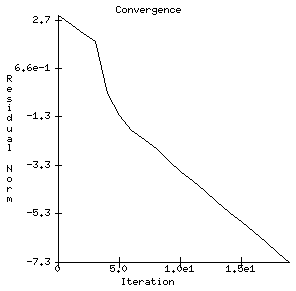
\includegraphics[width=0.9\textwidth]{line-graph-tri}
\caption{\PETSc can use X windows to produce line graphs at run time.  (This is not to say they are pretty.)}
\label{fig:line-graph-tri}
\end{marginfigure}

Finally, \PETSc can generate graphics showing convergence of iterative methods, at least if X11 windows are installed.  The line graph in Figure \ref{fig:line-graph-tri}, from
\begin{cline}
$ ./tri -tri_m 1000000 -ksp_rtol 1.0e-10 -pc_type jacobi \
    -ksp_monitor_lg_residualnorm -draw_pause 1
\end{cline}
%$
shows the residual norm logarithm versus the iteration number.

\bigskip
\section{Exercises}

\renewcommand{\labelenumi}{\arabic{chapter}.\arabic{enumi}\quad}
\begin{enumerate}
\item Suppose a square matrix $A$ with nonzero diagonal entries is decomposed into diagonal and lower/upper triangular parts as $A=D+L+U$.  Show that the Jacobi iteration $\bu_{k+1} = D^{-1} \left(\bb - L \bu_k - U \bu_k\right)$ is the same as the $\omega=1$ Richardson iteration \eqref{introrichardson} applied to the left-preconditioned system \eqref{introleftpre} with $M=D$.  Formulate and prove a corresponding statement about the Gauss-Seidel iteration $\bu_{k+1} = (D+L)^{-1} \left(\bb - U \bu_k\right)$.

\item Show \eqref{introconvergethm}.

\item Show \eqref{relativenormbounds}.
%For the left inequality, note first that $\|\br_0\| = \|\bb - A \bu_0\| \le \|A\| \|A^{-1} \bb - \bu\| = \|A\| \|\be_0\|$, and second that $\|\bu\| = \|A^{-1}\bb\| \le \|A^{-1}\| \|\bb\|$ so $1 / \|\bb\| \le \|A\| / \|\bu\|$.  Combining these gives the left inequality.

\item On page \pageref{krylovgoal} we note that a Krylov space approximation $p_{n-1}(A)\bb$ to the solution $A^{-1}\bb$ is close if $p_{n-1}(z)$ is close to $1/z$ on the spectrum of $A$.  Prove this for invertible diagonalizable matrices $A=S\Lambda S^{-1}$, with $\Lambda$ diagonal, by showing
	$$\|p_{n-1}(A) - A^{-1}\| \le \,\kappa(S)\, \max_{\lambda \in \sigma(A)} |p_{n-1}(\lambda) - \lambda^{-1}|$$
where $\kappa(S) = \|S\| \|S^{-1}\|$ is the condition number.\sidenote{Here $\|\cdot\|$ is any induced matrix norm \citep{TrefethenBau}.}  If $A$ is \emph{normal} then, by definition, $S$ can be chosen to be unitary.  In that case, using the $2$-norm, the condition number factor can have its minimal value of $1$.

\item For the $\omega=1$ Richardson iteration \eqref{introrichardson} and $\bu_0=\bb$ we get $\bu_k = q_k(A) \bb$ for polynomials $q_k$ given by \eqref{richpolys}.  Show that if $\lim_{k\to\infty} q_k=q_\infty$ exists then $q_\infty(x)=1/x$.  On the other hand, by setting $y=1-x$ and defining $Q_k(y)=q_k(1-y)$, show $Q_k(y)$ is the partial sum of a well-known series with a well-known radius of convergence.

\item Consider Richardson iteration in the example
\begin{cline}
./tri -tri_m 100 -ksp_monitor -ksp_type richardson
\end{cline}
Un-preconditioned Richardson iteration fails (i.e.~add \texttt{-pc\_type none}); explain.  The default preconditioner succeeds (i.e.~\texttt{-pc\_type ilu}), but ILU($0$) is cheating because it becomes a complete LU factorization on this tridiagonal and diagonally-dominant $A$; we are really seeing a direct solve.  The same can be said for ICC($0$).  Confirm that, as in the example on page \pageref{introprerichardson}, Richardson iteration succeeds with \texttt{-pc\_type jacobi}, even though the diagonal is constant; explain.

\item \label{exer:computeeigs} Un-preconditioned GMRES solves the linear system in \texttt{tri.c} reasonably efficiently.  We can explain this by asking \PETSc to compute the eigenvalues of $A$ by using option\sidenote{The relevant \PETSc manual page says this option is ``intended only for assistance in understanding the convergence of iterative methods, not for eigenanalysis.  For accurate computation of eigenvalues we recommend using the excellent package SLEPc.''  See \href{http://slepc.upv.es/}{\texttt{slepc.upv.es}}.}
\begin{quote}
\texttt{-ksp\_compute\_eigenvalues}
\end{quote}
Because otherwise it computes the eigenvalues of the preconditioned operator $P^{-1}A$, add \texttt{-pc\_type none}.  Try dimensions $N=10,100,1000$.  Why does the  run
\begin{cline}
./tri -tri_n 1000 -pc_type none -ksp_compute_eigenvalues
\end{cline}
only show 11 eigenvalues of this $1000\times 1000$ matrix?  How do these eigenvalues explain the good behavior of unpreconditioned GMRES?\sidenote{See \citep{TrefethenBau} for help with both of these questions.}

\item The accuracy of direct solves (e.g.~\texttt{-ksp\_type preonly -pc\_type cholesky}) in \texttt{tri.c}, as measured by the reported error norm $\|\bx - \bx_{\text{exact}}\|_2$, decreases with increasing dimension.  Confirm and explain this observation.

\item Table \ref{tab:tritiming} includes a number of blanks.  For each one, explain why it is blank, experimenting if needed.

\item Table \ref{tab:tritiming} gives execution times not iteration count.  Generate the corresponding table of \pKSP iteration count by adding option \verb|-ksp_converged_reason| to the run commands.  Note the large number of ``coincidences'' in iteration count, i.e.~cases where iteration counts are identical; explain.  Which preconditioners have a strong or weak effect on iteration count?  Is timing or iteration count more useful?

\item As the reader will undoubtedly experience, segmentation faults and memory leaks are inevitable when one develops \PETSc codes.  A standard tool for detecting/diagnosing these is \texttt{valgrind}.\sidenote{See \href{http://valgrind.org/}{\texttt{valgrind.org}}.}  We recommend running it frequently.  As an exercise, run
\begin{cline}
valgrind ./vecmatksp
\end{cline}
to see what \texttt{valgrind} shows for a leak-free program.  Then comment-out a \texttt{VecDestroy()} call in \texttt{vecmatksp.c} and rerun to see a common type of memory leak.

% from Barry Smith on petsc-users: "What does your -log_summary output look like? One thing that GMRES does is it introduces a global reduction with each multiple (hence a barrier across all your processes) on some systems this can be deadly."  Turn this into GMRES exercise on many processors with tri.c?

\end{enumerate}
